% Options for packages loaded elsewhere
\PassOptionsToPackage{unicode}{hyperref}
\PassOptionsToPackage{hyphens}{url}
\PassOptionsToPackage{dvipsnames,svgnames*,x11names*}{xcolor}
%
\documentclass[
  8pt,
  ignorenonframetext,
  dvipsnames]{beamer}
\usepackage{pgfpages}
\setbeamertemplate{caption}[numbered]
\setbeamertemplate{caption label separator}{: }
\setbeamercolor{caption name}{fg=normal text.fg}
\beamertemplatenavigationsymbolsempty
% Prevent slide breaks in the middle of a paragraph
\widowpenalties 1 10000
\raggedbottom
\setbeamertemplate{part page}{
  \centering
  \begin{beamercolorbox}[sep=16pt,center]{part title}
    \usebeamerfont{part title}\insertpart\par
  \end{beamercolorbox}
}
\setbeamertemplate{section page}{
  \centering
  \begin{beamercolorbox}[sep=12pt,center]{part title}
    \usebeamerfont{section title}\insertsection\par
  \end{beamercolorbox}
}
\setbeamertemplate{subsection page}{
  \centering
  \begin{beamercolorbox}[sep=8pt,center]{part title}
    \usebeamerfont{subsection title}\insertsubsection\par
  \end{beamercolorbox}
}
\AtBeginPart{
  \frame{\partpage}
}
\AtBeginSection{
  \ifbibliography
  \else
    \frame{\sectionpage}
  \fi
}
\AtBeginSubsection{
  \frame{\subsectionpage}
}
\usepackage{lmodern}
\usepackage{amssymb,amsmath}
\usepackage{ifxetex,ifluatex}
\ifnum 0\ifxetex 1\fi\ifluatex 1\fi=0 % if pdftex
  \usepackage[T1]{fontenc}
  \usepackage[utf8]{inputenc}
  \usepackage{textcomp} % provide euro and other symbols
\else % if luatex or xetex
  \usepackage{unicode-math}
  \defaultfontfeatures{Scale=MatchLowercase}
  \defaultfontfeatures[\rmfamily]{Ligatures=TeX,Scale=1}
\fi
% Use upquote if available, for straight quotes in verbatim environments
\IfFileExists{upquote.sty}{\usepackage{upquote}}{}
\IfFileExists{microtype.sty}{% use microtype if available
  \usepackage[]{microtype}
  \UseMicrotypeSet[protrusion]{basicmath} % disable protrusion for tt fonts
}{}
\makeatletter
\@ifundefined{KOMAClassName}{% if non-KOMA class
  \IfFileExists{parskip.sty}{%
    \usepackage{parskip}
  }{% else
    \setlength{\parindent}{0pt}
    \setlength{\parskip}{6pt plus 2pt minus 1pt}}
}{% if KOMA class
  \KOMAoptions{parskip=half}}
\makeatother
\usepackage{xcolor}
\IfFileExists{xurl.sty}{\usepackage{xurl}}{} % add URL line breaks if available
\IfFileExists{bookmark.sty}{\usepackage{bookmark}}{\usepackage{hyperref}}
\hypersetup{
  pdftitle={Introduction to Multivariate Regression \& Econometrics},
  pdfauthor={Lecture 10},
  colorlinks=true,
  linkcolor=Maroon,
  filecolor=Maroon,
  citecolor=Blue,
  urlcolor=blue,
  pdfcreator={LaTeX via pandoc}}
\urlstyle{same} % disable monospaced font for URLs
\newif\ifbibliography
\usepackage{graphicx,grffile}
\makeatletter
\def\maxwidth{\ifdim\Gin@nat@width>\linewidth\linewidth\else\Gin@nat@width\fi}
\def\maxheight{\ifdim\Gin@nat@height>\textheight\textheight\else\Gin@nat@height\fi}
\makeatother
% Scale images if necessary, so that they will not overflow the page
% margins by default, and it is still possible to overwrite the defaults
% using explicit options in \includegraphics[width, height, ...]{}
\setkeys{Gin}{width=\maxwidth,height=\maxheight,keepaspectratio}
% Set default figure placement to htbp
\makeatletter
\def\fps@figure{htbp}
\makeatother
\setlength{\emergencystretch}{3em} % prevent overfull lines
\providecommand{\tightlist}{%
  \setlength{\itemsep}{0pt}\setlength{\parskip}{0pt}}
\setcounter{secnumdepth}{-\maxdimen} % remove section numbering

%packages
\usepackage{graphicx}
\usepackage{rotating}
\usepackage{hyperref}

\usepackage{tikz} % used for text highlighting, amongst others
\usepackage{comment}

%title slide stuff
%\institute{Department of Education}
%\title{Managing and Manipulating Data Using R}

%
\setbeamertemplate{navigation symbols}{} % get rid of navigation icons:
\setbeamertemplate{footline}[page number]

%\setbeamertemplate{frametitle}{\thesection \hspace{0.2cm} \insertframetitle}
\setbeamertemplate{section in toc}[sections numbered]
%\setbeamertemplate{subsection in toc}[subsections numbered]
\setbeamertemplate{subsection in toc}{%
  \leavevmode\leftskip=3.2em\color{gray}\rlap{\hskip-2em\inserttocsectionnumber.\inserttocsubsectionnumber}\inserttocsubsection\par
}

%define colors
%\definecolor{uva_orange}{RGB}{216,141,42} % UVa orange (Rotunda orange)
\definecolor{mygray}{rgb}{0.95, 0.95, 0.95} % for highlighted text
	% grey is equal parts red, green, blue. higher values >> lighter grey
	%\definecolor{lightgraybo}{rgb}{0.83, 0.83, 0.83}

% new commands

%highlight text with very light grey
\newcommand*{\hlg}[1]{%
	\tikz[baseline=(X.base)] \node[rectangle, fill=mygray] (X) {#1};%
}
%, inner sep=0.3mm
%highlight text with very light grey and use font associated with code
\newcommand*{\hlgc}[1]{\texttt{\hlg{#1}}}

%modifying back ticks to add grey background
\let\OldTexttt\texttt
\renewcommand{\texttt}[1]{\OldTexttt{\hlg{#1}}}


\begin{comment}

% Font
\usepackage[defaultfam,light,tabular,lining]{montserrat}
\usepackage[T1]{fontenc}
\renewcommand*\oldstylenums[1]{{\fontfamily{Montserrat-TOsF}\selectfont #1}}

% Change color of boldface text to darkgray
\renewcommand{\textbf}[1]{{\color{darkgray}\bfseries\fontfamily{Montserrat-TOsF}#1}}

% Bullet points
\setbeamertemplate{itemize item}{\color{BlueViolet}$\circ$}
\setbeamertemplate{itemize subitem}{\color{BrickRed}$\triangleright$}
\setbeamertemplate{itemize subsubitem}{$-$}

% Reduce space before lists
%\addtobeamertemplate{itemize/enumerate body begin}{}{\vspace*{-8pt}}

\let\olditem\item
\renewcommand{\item}{%
  \olditem\vspace{4pt}
}

% decreasing space before and after level-2 bullet block
%\addtobeamertemplate{itemize/enumerate subbody begin}{}{\vspace*{-3pt}}
%\addtobeamertemplate{itemize/enumerate subbody end}{}{\vspace*{-3pt}}

% decreasing space before and after level-3 bullet block
%\addtobeamertemplate{itemize/enumerate subsubbody begin}{}{\vspace*{-2pt}}
%\addtobeamertemplate{itemize/enumerate subsubbody end}{}{\vspace*{-2pt}}

%Section numbering
\setbeamertemplate{section page}{%
    \begingroup
        \begin{beamercolorbox}[sep=10pt,center,rounded=true,shadow=true]{section title}
        \usebeamerfont{section title}\thesection~\insertsection\par
        \end{beamercolorbox}
    \endgroup
}

\setbeamertemplate{subsection page}{%
    \begingroup
        \begin{beamercolorbox}[sep=6pt,center,rounded=true,shadow=true]{subsection title}
        \usebeamerfont{subsection title}\thesection.\thesubsection~\insertsubsection\par
        \end{beamercolorbox}
    \endgroup
}

\end{comment}

\title{Introduction to Multivariate Regression \& Econometrics}
\subtitle{HED 612}
\author{Lecture 10}
\date{}

\begin{document}
\frame{\titlepage}

\begin{frame}
  \tableofcontents[hideallsubsections]
\end{frame}
\begin{frame}{Where are we going\ldots.}
\protect\hypertarget{where-are-we-going.}{}

\begin{itemize}
\tightlist
\item
  This Lecture

  \begin{itemize}
  \tightlist
  \item
    Introduction to multivariate regression
  \item
    Introduction to reading methods/results sections for empirical
    articles
  \end{itemize}
\item
  Homework and Reading

  \begin{itemize}
  \tightlist
  \item
    Problem Set \#10
  \item
    Reading for next Lecture:

    \begin{itemize}
    \tightlist
    \item
      Powers, J. M. (2004). High-Stakes Accountability and Equity: Using
      Evidence From California's Public Schools Accountability Act to
      Address the Issues in Williams v. State of California.
      \emph{American Educational Research Journal}, 41(4), 763--795.
    \end{itemize}
  \end{itemize}
\item
  Next Lecture

  \begin{itemize}
  \tightlist
  \item
    Other OLS assumptions
  \item
    Graphing multivariate regression results
  \item
    Creating publication quality tables
  \end{itemize}
\item
  Next Next Lecture

  \begin{itemize}
  \tightlist
  \item
    Introduction to non-linear relationships between X and Y
  \item
    Mini lesson on what each section of manuscript should accomplish!
  \end{itemize}
\end{itemize}

\end{frame}

\hypertarget{introduction-to-multivariate-regression}{%
\section{Introduction to Multivariate
Regression}\label{introduction-to-multivariate-regression}}

\begin{frame}{Population Regression Model}
\protect\hypertarget{population-regression-model}{}

\begin{itemize}
\tightlist
\item
  Same as in ``simple'' (bivariate) regression; we just add more
  regressors (i.e., independent/control variables) into our model!
\end{itemize}

\medskip

Population Regression Model

\begin{itemize}
\tightlist
\item
  \(Y_i = \beta_0 + \beta_1X_{1i} + \beta_2X_{2i} +\) \ldots{}
  \(\beta_kX_{ki} + u_i\)
\item
  Where:

  \begin{itemize}
  \tightlist
  \item
    \(Y_i\) = observation i of dependent variable
  \item
    \(X_{1i}\) = observation i of the \textbf{first regressor}, \(X_1\)
  \item
    \(X_{2i}\) = observation i of the \textbf{second regressor}, \(X_2\)
  \item
    \(X_{ki}\) = observation i of the \textbf{Kth regressor}, \(X_k\)
  \item
    \(\beta_1\) = population average effect of Y for ``change'' in
    \(X_1\)

    \begin{itemize}
    \tightlist
    \item
      if \(X_1\) is continuous: average effect of Y for one-unit
      increase/decrease in \(X_1\)
    \item
      if \(X_1\) is categorical: population average effect of being in
      the non-reference group as opposed to the reference group
    \end{itemize}
  \item
    \(\beta_2\) = population average effect of Y for ``change'' in
    \(X_2\)
  \item
    \(\beta_k\) = population average effect of Y for ``change'' \(X_k\)
  \item
    \(\beta_0\) = average value of Y when the value of \emph{all
    independent variables (\(X_1, X_2 ...X_k\)) are equal to zero}
  \item
    \(u_i\) = all other variables that affect the value of \(Y_i\) but
    are not included in the model
  \end{itemize}
\end{itemize}

\end{frame}

\begin{frame}{Things we do in regression; all work the same in
multivariate!}
\protect\hypertarget{things-we-do-in-regression-all-work-the-same-in-multivariate}{}

\begin{enumerate}
\tightlist
\item
  Estimation
\end{enumerate}

\begin{itemize}
\tightlist
\item
  Choose estimates for \(\beta_0, \beta_1, \beta_2, ... \beta_k\) by
  selecting those that minimize the sum of squared errors (i.e., make
  the best prediction of Y), yielding an OLS line

  \begin{itemize}
  \tightlist
  \item
    \(\hat{Y_i} = \hat{\beta_0} + \hat{\beta_1} X_{1i} + \hat{\beta_2} X_{2i} + ... \hat{\beta_k} X_{ki}\)
  \end{itemize}
\end{itemize}

\begin{enumerate}
\setcounter{enumi}{1}
\tightlist
\item
  Measures of model fit (e.g., \(R^2\), SER)
\end{enumerate}

\begin{itemize}
\tightlist
\item
  But formulas change slightly to account for degrees of freedom!
\item
  Once you introduce multiple independent variables, use adjusted
  R-squared
\item
  Adjusted R-squared

  \begin{itemize}
  \tightlist
  \item
    Adjusted for the number of predictors in the model
  \item
    Every independent variable we add to the model will increase our
    ``normal'' R-squared; but doesn't necessarily mean it's a better
    fit!
  \item
    Adjusted R squared increases only if new variable improves the model
    more than would be expected by chance!
  \end{itemize}
\end{itemize}

\begin{enumerate}
\setcounter{enumi}{2}
\tightlist
\item
  Prediction
\end{enumerate}

\begin{itemize}
\tightlist
\item
  Once you estimate OLS regression line, we can calculate predicted
  values for observations with particular values of all independent
  variables

  \begin{itemize}
  \tightlist
  \item
    \(\hat{Y_i} = \hat{\beta_0} + \hat{\beta_1} X_{1i} + \hat{\beta_2} X_{2i} + ... \hat{\beta_k} X_{ki}\)
  \end{itemize}
\end{itemize}

\begin{enumerate}
\setcounter{enumi}{3}
\tightlist
\item
  Hypothesis testing and confidence intervals about \(\beta_1\)
\end{enumerate}

\begin{itemize}
\tightlist
\item
  Same as before but formulas for \(\hat{\beta_1}\) and
  \(SE(\hat{\beta_1})\) change slightly, but R calculates this for us!
\end{itemize}

\end{frame}

\begin{frame}{OLS Assumption 1: Conditional Independence Assumption}
\protect\hypertarget{ols-assumption-1-conditional-independence-assumption}{}

\begin{itemize}
\tightlist
\item
  OLS Assumption 1 (in words)

  \begin{itemize}
  \tightlist
  \item
    the independent variable \(X_i\) is unrelated to the ``other
    variables'' not included in the model, \(u_i\)
  \end{itemize}
\item
  OLS Assumption 1 (mathematically)

  \begin{itemize}
  \tightlist
  \item
    \(E(u_i|X_i)=0\); the expected value of \(u_i\), given any value of
    \(X_i\), equals zero
  \end{itemize}
\item
  Multivariate regression helps us meet the conditional independence
  assumption

  \begin{itemize}
  \tightlist
  \item
    In other words, we add variables into our model that if left out
    would violate the conditional independence assumption and bias our
    \(\hat{\beta_1}\)
  \end{itemize}
\item
  Example: What is the effect of participating in Mexican American
  Studies program (MAS) on academic achievement?

  \begin{itemize}
  \tightlist
  \item
    We have to account for the fact that students choose to participate
    in MAS (self-selection bias); they were not randomly assigned to
    participate versus not participate in MAS!
  \end{itemize}
\end{itemize}

\end{frame}

\begin{frame}{OLS Assumption 1: Conditional Independence Assumption}
\protect\hypertarget{ols-assumption-1-conditional-independence-assumption-1}{}

\begin{itemize}
\tightlist
\item
  What is the effect of participation in MAS on high school graduation?
\item
  \(Y_i = \beta_0 + \beta_1X_{1i} + \beta_2X_{2i} + \beta_3X_{3i} + u_i\)
\item
  Where:

  \begin{itemize}
  \tightlist
  \item
    Y= GPA
  \item
    X1 = 0/1 MAS participation {[}non-reference group{]}; Did not
    participate in MAS {[}reference group{]}
  \item
    X2= previous academic achievement
  \item
    X3= socioeconomic status
  \end{itemize}
\item
  \textbf{Conditional independence assumption}:

  \begin{itemize}
  \tightlist
  \item
    Once we include control variables, there are no longer any omitted
    variables, Z, that satisfy \emph{both} of these two conditions:

    \begin{enumerate}
    [(1)]
    \tightlist
    \item
      Z affects value of Y \emph{and}
    \item
      Z has a relationship with X
    \end{enumerate}
  \end{itemize}
\item
  If we satisfy the conditional independence assumption through control
  variables, then multivariate regression is just as good as randomized
  assignment experiment!

  \begin{itemize}
  \tightlist
  \item
    Warning: But we often don't have every single control variable we
    need, so we get as close as possible!
  \end{itemize}
\end{itemize}

\end{frame}

\begin{frame}{Multivariate regression in Econometrics vs Social Science}
\protect\hypertarget{multivariate-regression-in-econometrics-vs-social-science}{}

\begin{itemize}
\tightlist
\item
  \(Y_i = \beta_0 + \beta_1X_{1i} + \beta_2X_{2i} + \beta_3X_{3i} + u_i\)
\item
  Econometrics

  \begin{itemize}
  \tightlist
  \item
    We are only interested in estimating \(\beta_1\) {[}the causal
    effect of \(X_{1i}\) on Y{]}
  \item
    The only reason we include other variables in the model besides X1
    is to eliminate omitted variable bias
  \item
    Therefore, we include all control variables that satisfy \emph{both}
    conditions of omitted variable bias
  \item
    Once we include control variables, and no other variables satisfy
    both conditions, then we satisfy the conditional independence
    assumption and we can estimate a causal effect!
  \end{itemize}
\item
  Traditional social science statistics {[}most of my research!{]}

  \begin{itemize}
  \tightlist
  \item
    Purpose of multiple regression is to add new variable to your model
    (e.g., \(X_3\)) to see the effect of \(X_3\) on Y
  \item
    Can lead to sloppy research if we take a ``throw'' everything and
    the kitchen sink into a model and see what's interesting!
  \item
    We'll read some good examples of this type of research including our
    first empirical article next week:

    \begin{itemize}
    \tightlist
    \item
      Powers (2004)
    \end{itemize}
  \end{itemize}
\end{itemize}

\end{frame}

\begin{frame}{Multivariate regression in R}
\protect\hypertarget{multivariate-regression-in-r}{}

\begin{itemize}
\tightlist
\item
  Research question: What is the effect of student teacher ratio on
  student reading test scores?
\item
  \textbf{Simple/Bivariate regression}

  \begin{itemize}
  \tightlist
  \item
    \(Y_i = \beta_0 + \beta_1X_{1i} + u_i\)
  \item
    Where:

    \begin{itemize}
    \tightlist
    \item
      Y= reading test scores
    \item
      \(X_1\) = student teacher ratio
    \end{itemize}
  \item
    General interpretation of \(\hat{\beta_1}\): The average effect of a
    one-unit increase in \(X_1\) is associated with a \(\hat{\beta_1}\)
    change in Y

    \begin{itemize}
    \tightlist
    \item
      The average effect of a one-unit increase in student teacher ratio
      is associated with a 2.62 decrease in district average reading
      test scores
    \end{itemize}
  \end{itemize}
\item
  \textbf{Multivariate regression}

  \begin{itemize}
  \tightlist
  \item
    \(Y_i = \beta_0 + \beta_1X_{1i} + \beta_2X_{2i} + u_i\)
  \item
    Where:

    \begin{itemize}
    \tightlist
    \item
      Y= student test scores
    \item
      \(X_1\) = student teacher ratio
    \item
      \(X_2\) = \% ELL {[}from last week, established \%ELL meets both
      conditions of omitted variable bias{]}
    \end{itemize}
  \item
    General interpretation of \(\hat{\beta_1}\): The average effect of a
    one-unit increase in \(X_1\) is associated with a \(\hat{\beta_1}\)
    change in Y, \textbf{holding the value of \(X_2\) constant}

    \begin{itemize}
    \tightlist
    \item
      The average effect of a one-unit increase in student teacher ratio
      is associated with a 1.29 decrease in district average reading
      test scores, \textbf{holding the value of \%ELL students constant}
    \end{itemize}
  \end{itemize}
\end{itemize}

\end{frame}

\begin{frame}{What does ``holding constant'' mean?}
\protect\hypertarget{what-does-holding-constant-mean}{}

\begin{itemize}
\tightlist
\item
  RQ: What is the effect of student teacher ratio on reading test
  scores?

  \begin{itemize}
  \tightlist
  \item
    \(Y_i = \beta_0 + \beta_1X_{1i} + \beta_2X_{2i} + u_i\)
  \item
    Where: Y= student test scores, \(X_1\) = student teacher ratio,
    \(X_2\) = \% ELL
  \end{itemize}
\item
  Setup:

  \begin{itemize}
  \tightlist
  \item
    We think student test scores go down if there's a greater percentage
    of ELL students in the classroom

    \begin{itemize}
    \tightlist
    \item
      First condition of omitted variable bias ( Z affects Y)
    \end{itemize}
  \item
    We think there is a negative relationship between percentage of ELL
    students in the classroom and student-teacher ratio

    \begin{itemize}
    \tightlist
    \item
      Second condition of omitted variable bias ( Z has a relationship
      with X)
    \end{itemize}
  \end{itemize}
\item
  Problem:

  \begin{itemize}
  \tightlist
  \item
    We think student teacher ratio and percentage of ELL move together
  \item
    We want to know the relationship between reading scores and student
    teacher ratio when ``percent ELL'' is not allowed to move!
  \end{itemize}
\item
  ``Holding the value of \(X_2\) constant''

  \begin{itemize}
  \tightlist
  \item
    Means to estimate the relationship between \(X_1\) and Y when we
    don't allow the value of \(X_2\) to vary
  \item
    In other words, we analyze the relationship between student teacher
    ration (\(X_1\)) and reading test scores (Y) for applicants that
    have the same value of percent ELL (\(X_2\)) {[}calculus: partial
    derivatives!{]}
  \end{itemize}
\end{itemize}

\end{frame}

\begin{frame}{What does ``holding constant'' mean? Another
example\ldots.}
\protect\hypertarget{what-does-holding-constant-mean-another-example.}{}

\begin{itemize}
\tightlist
\item
  RQ: What is the relationship between years of education(X1) on
  income(Y), after controlling for years of work experience (X2)?
\item
  General interpretation of \(\hat{\beta_1}\):

  \begin{itemize}
  \tightlist
  \item
    The average effect of a one-unit increase in X1 is a
    \(\hat{\beta_1}\) unit increase in Y, holding the value of X2
    constant
  \end{itemize}
\item
  Interpretation of \(\hat{\beta_1}\), applied to example

  \begin{itemize}
  \tightlist
  \item
    The effect of having one additional year of education (X1) on income
    (Y), when we don't allow value of ``years of experience'' (X2) to
    change
  \item
    Compare people with 2 years of college versus 3 years of college
    that have the same years experience to assess the ``effect'' of an
    additional year of education on income
  \end{itemize}
\item
  Said differently: analyze the effect of increasing years of education
  on income for people who have same years of experience
\end{itemize}

\end{frame}

\begin{frame}{Interpreting \(\hat{\beta_1}\) for continuous X}
\protect\hypertarget{interpreting-hatbeta_1-for-continuous-x}{}

\begin{itemize}
\tightlist
\item
  RQ: What is the effect of student teacher ratio (X1) on average
  district reading test scores (X2)?

  \begin{itemize}
  \tightlist
  \item
    \(Y_i = \beta_0 + \beta_1X_{1i} + \beta_2X_{2i} + \beta_3X_{3i} + u_i\)
  \item
    Where:

    \begin{itemize}
    \tightlist
    \item
      Y= reading test scores
    \item
      \(X_1\) = average district student teacher ratio
    \item
      \(X_2\) = 0/1 majority ELL district {[}greater than 50\% ELL
      students= non-reference group; less than 50\% ELL
      students=reference group{]}
    \item
      \(X_3\) = avg district income (\$000s)
    \end{itemize}
  \end{itemize}
\item
  General interpretation of \(\hat{\beta_1}\) for continuous X {[}all
  are correct/same{]}

  \begin{itemize}
  \tightlist
  \item
    The average effect of a one unit increase in \(X_1\) is a
    \(\hat{\beta_1}\) unit change in Y, holding the values of \(X_2\)
    and \(X_3\) constant
  \item
    OR The average effect of a one unit increase in \(X_1\) is a
    \(\hat{\beta_1}\) unit change in Y, after controlling for \(X_2\)
    and \(X_3\)
  \item
    The average effect of a one unit increase in \(X_1\) is a
    \(\hat{\beta_1}\) unit change in Y, holding the values of covariates
    constant
  \end{itemize}
\item
  Run regression in R!
\item
  \(\hat{Y_i} = \hat{\beta_0} + \hat{\beta_1} X_{1i} + \hat{\beta_2} X_{2i} + \hat{\beta_3} X_{3i}\)
\item
  \(\hat{Y_i} = 646.2 - 0.8 X_{1i} -23.5 X_{2i} + 1.7 X_{3i}\)
\item
  Specific example interpretation {[}run regression in R{]}

  \begin{itemize}
  \tightlist
  \item
    The average effect of a one-unit increase in average district
    student teacher ratio (i.e., one additional student per teacher) is
    a 0.8 point decrease in average district reading score, holding the
    values of majority ELL and district average income constant
  \end{itemize}
\end{itemize}

\end{frame}

\begin{frame}[fragile]{Interpreting \(\hat{\beta_1}\) for categorical X}
\protect\hypertarget{interpreting-hatbeta_1-for-categorical-x}{}

\begin{itemize}
\tightlist
\item
  RQ: What is the effect of being a majority ELL district (X1) on
  average district reading test scores (X2)?

  \begin{itemize}
  \tightlist
  \item
    \(Y_i = \beta_0 + \beta_1X_{1i} + \beta_2X_{2i} + \beta_3X_{3i} + u_i\)
  \item
    Where:

    \begin{itemize}
    \tightlist
    \item
      Y= reading test scores
    \item
      \(X_1\) = 0/1 majority ELL {[}non-reference group{]}, \(X_2\) =
      avg district student teacher ratio; \(X_3\) = avg district income
      (\$000s)
    \end{itemize}
  \item
    \textbf{Stylistic Note}: Your main independent variable of interest
    should always be \(X_1\)
  \end{itemize}
\item
  General interpretation of \(\hat{\beta_1}\) for categorical X

  \begin{itemize}
  \tightlist
  \item
    Being {[}non-reference group{]} as opposed to {[}reference group{]}
    is associated with a \(\hat{\beta_1}\) unit change in Y, holding the
    values of \(X_2\) and \(X_3\) constant
  \end{itemize}
\item
  Run regression in R {[}note: same coef values as previous model but in
  diff order!{]}

  \begin{itemize}
  \tightlist
  \item
    \(\hat{Y_i} = \hat{\beta_0} + \hat{\beta_1} X_{1i} + \hat{\beta_2} X_{2i} + \hat{\beta_3} X_{3i}\)
  \item
    \(\hat{Y_i} = 646.2 - 23.5 X_{1i} -0.8 X_{2i} + 1.7 X_{3i}\)
  \end{itemize}
\item
  Specific interpretation

  \begin{itemize}
  \tightlist
  \item
    Reference group vs non Reference group

    \begin{itemize}
    \tightlist
    \item
      0 = non-ELL majority district {[}lowest value is automatically
      removed from regression as reference group{]}
    \item
      1 = majority ELL district {[}non-reference group is kept within
      regression; this is why the regression output coefficient says
      \textbf{\texttt{ell1}}{]}
    \end{itemize}
  \item
    Being a majority ELL district as opposed to a non-majority ELL
    district is associated with a 23.5 point decrease in average
    district reading scores, holding values of average student-teacher
    ratio and district average income constant
  \end{itemize}
\end{itemize}

\end{frame}

\begin{frame}{Prediction still works the same way!}
\protect\hypertarget{prediction-still-works-the-same-way}{}

\begin{itemize}
\tightlist
\item
  RQ: What is the effect of being a majority ELL district (X1) on
  average district reading test scores (X2)?

  \begin{itemize}
  \tightlist
  \item
    \(Y_i = \beta_0 + \beta_1X_{1i} + \beta_2X_{2i} + \beta_3X_{3i} + u_i\)
  \item
    Where:

    \begin{itemize}
    \tightlist
    \item
      Y= reading test scores
    \item
      \(X_1\) = 0/1 majority ELL district
    \item
      \(X_2\) = avg district student teacher ratio
    \item
      \(X_3\) = avg district income (\$000s)
    \end{itemize}
  \end{itemize}
\item
  Run regression in R

  \begin{itemize}
  \tightlist
  \item
    \(\hat{Y_i} = \hat{\beta_0} + \hat{\beta_1} X_{1i} + \hat{\beta_2} X_{2i} + \hat{\beta_3} X_{3i}\)
  \item
    \(\hat{Y_i} = 646.2 - 23.5 X_{1i} -0.8 X_{2i} + 1.7 X_{3i}\)
  \end{itemize}
\item
  What's the predicted average reading score for a district that is a
  non-ELL majority district, has a student teacher ratio of 25, and
  average district income of \$22,000?

  \begin{itemize}
  \tightlist
  \item
    \((Y| X_1=0, X_2=25, X_3=22)\) = 646.2 - (23.5 * 0) - (0.8 * 25) +
    (1.7 * 22)
  \item
    \((Y| X_1=0, X_2=25, X_3=22)\) = 646.2 - (0) - (20) + (37.4)
  \item
    \((Y| X_1=0, X_2=25, X_3=22)\) = 663.6
  \end{itemize}
\item
  What's the predicted average reading score for a district that is an
  ELL majority district, has a student teacher ratio of 19, and average
  district income of \$26,000?

  \begin{itemize}
  \tightlist
  \item
    \((Y| X_1=1, X_2=19, X_3=26)\) = 646.2 - (23.5 * 1) - (0.8 * 19) +
    (1.7 * 26)
  \item
    \((Y| X_1=1, X_2=19, X_3=26)\) = 646.2 - (23.5) - (15.2) + (44.2)
  \item
    \((Y| X_1=1, X_2=19, X_3=26)\) = 651.7
  \end{itemize}
\end{itemize}

\end{frame}

\hypertarget{reading-empirical-regression-results}{%
\section{Reading Empirical Regression
Results}\label{reading-empirical-regression-results}}

\begin{frame}{Our first example of empirical regression results}
\protect\hypertarget{our-first-example-of-empirical-regression-results}{}

Powers, J. M. (2004). High-Stakes Accountability and Equity: Using
Evidence From California's Public Schools Accountability Act to Address
the Issues in Williams v. State of California. \emph{American
Educational Research Journal}, 41(4), 763--795.

\medskip

\begin{itemize}
\tightlist
\item
  RQ: What is relationship between school resource variables and
  school-level academic performance index (API)?
\item
  Does not frame article as ``causal inference'' but Powers is doing
  exactly what we have learned in this lecture/class!

  \begin{itemize}
  \tightlist
  \item
    Attempts to analyze the effect of school resources (X) on the
    academic achievement of schools (Y) by controlling for variables
    that would be ``systematically related'' to the independent
    variables of interest and have an effect on the dependent variable
  \item
    Does not have all possible controls to get to a ``causal effect''
    equivalent to what we would estimate if the study was designed as an
    randomized control experiment.
  \end{itemize}
\end{itemize}

\end{frame}

\begin{frame}[fragile]{How to read a methods section\ldots{}}
\protect\hypertarget{how-to-read-a-methods-section}{}

\begin{itemize}
\tightlist
\item
  The format of quantitative empirical research is pretty
  ``standardized'', which makes it easy to read as you get more
  experience\ldots{}
\item
  Methods section usually outlines the data used, sample, variables, and
  the methods used
\end{itemize}

\medskip

For Powers (2004):

\begin{itemize}
\tightlist
\item
  Data: uses data similar to our \texttt{caschools} (ours is district
  level; Powers uses school-level!)
\item
  Sample: All CA schools that were assigned an API score

  \begin{itemize}
  \tightlist
  \item
    97\% of full population of CA schools
  \end{itemize}
\item
  Variables: provides details on all the variables in the model!

  \begin{itemize}
  \tightlist
  \item
    Pay attention to how variables are constructed!
  \item
    Note that sometimes we don't have a variable we need, so we use a
    ``proxy.'' It's the authors' responsibility to convince readers why
    the variable used is a good enough proxy for the unavailable
    variable needed
  \item
    Empirical studies use a lot of variables in the model which are
    difficult to keep track of; so they are often ``grouped'' into
    categories (e.g., student characteristics, school resources, etc)
  \end{itemize}
\item
  Methodology: This section varies depending on the sophistication of
  the method.

  \begin{itemize}
  \tightlist
  \item
    Sometimes they write out the full population regression model,
    sometimes they don't
  \item
    Linear regression is considered simple so in most cases they don't
  \end{itemize}
\end{itemize}

\end{frame}

\begin{frame}{How to read results (descriptives)\ldots{}}
\protect\hypertarget{how-to-read-results-descriptives}{}

\begin{itemize}
\tightlist
\item
  Quantitative research studies \textbf{nearly always} present the
  descriptive statistics of all variables used in a table

  \begin{itemize}
  \tightlist
  \item
    In most cases the mean and standard deviation is sufficient; if it's
    substantively important sometimes min and max (or can be covered
    within text of the variables sub-section of the methods section)
  \item
    Sometimes authors dedicate space within text to explaining
    descriptive stats and sometimes they don't

    \begin{itemize}
    \tightlist
    \item
      Usually depends on how substantively important they are\ldots{}
    \item
      Most folks can read the table so authors will avoid spending too
      much limited space on descriptive statistics
    \end{itemize}
  \end{itemize}
\end{itemize}

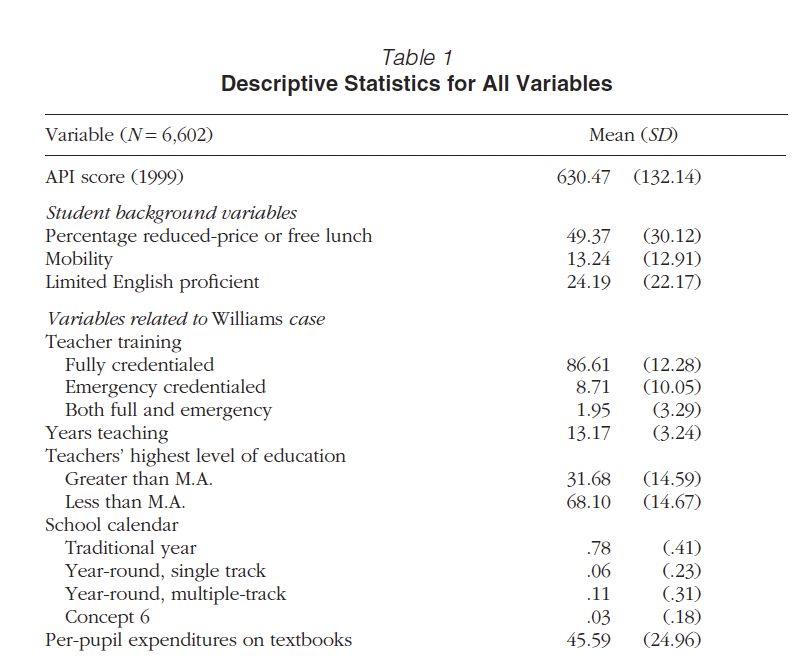
\includegraphics{powers_table1.png}

\end{frame}

\begin{frame}{How to read results (regression models)\ldots{}}
\protect\hypertarget{how-to-read-results-regression-models}{}

\begin{itemize}
\tightlist
\item
  The way in which regression results are presented is well standardized
  across all fields and journals! {[}some exceptions{]}
\item
  Regression tables usually show the beta coefficient and standard error
  (usually in parentheses) for each independent variable
\item
  Columns are individual models!

  \begin{itemize}
  \tightlist
  \item
    Tables usually start with a simple regression model in the first
    column that only includes the main independent variable(s) of
    interest: ``model 1''
  \item
    Then add control variables incrementally; sometimes done in
    groupings
  \item
    This allows the author to show the ``progression'' in the models as
    variables are added in (particularly important for descriptive
    research to see changes in model fit statistics)
  \item
    Although, sometimes models in separate columns can also indicate
    various samples; look at the headings/read the authors description
    of table!
  \end{itemize}
\item
  Read the table notes!

  \begin{itemize}
  \tightlist
  \item
    Provide the key for interpreting the significance levels of p-values
    as denoted by asterisks ( \(*p\le 0.05\),
    \(**p\le 0.01\),\(***p\le 0.001\) )
  \item
    Will also tell you what the reference category is for categorical
    variables!
  \item
    Other useful information
  \end{itemize}
\end{itemize}

\end{frame}

\begin{frame}{How to read results (regression models)\ldots{}}
\protect\hypertarget{how-to-read-results-regression-models-1}{}

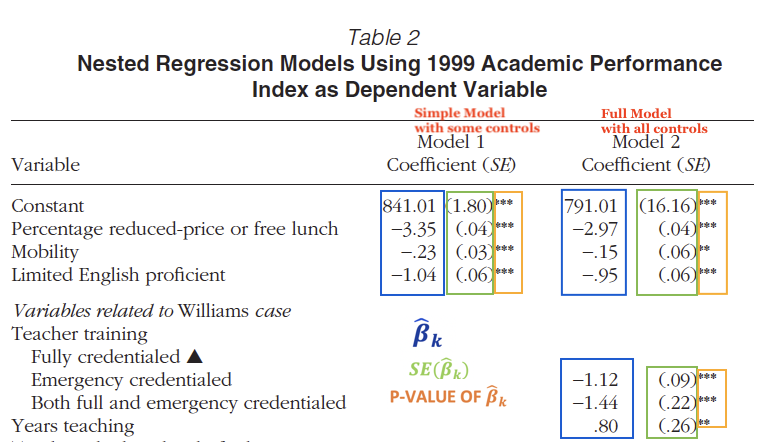
\includegraphics{POWERS_REGTABLE.png}

\end{frame}

\end{document}
